\let\negmedspace\undefined
\let\negthickspace\undefined
\documentclass[journal,12pt,onecolumn]{IEEEtran}
\usepackage{cite}
\usepackage{amsmath,amssymb,amsfonts,amsthm}
\usepackage{amsmath}
\usepackage{algorithmic}
\usepackage{graphicx}
\usepackage{textcomp}
\usepackage{xcolor}
\usepackage{txfonts}
\usepackage{listings}
\usepackage{multicol}
\usepackage{enumitem}
\usepackage{mathtools}
\usepackage{gensymb}
\usepackage{comment}
\usepackage[breaklinks=true]{hyperref}
\usepackage{tkz-euclide} 
\usepackage{listings}
\usepackage{gvv}                                        
\usepackage[latin1]{inputenc}                                
\usepackage{color}                                            
\usepackage{array}                                            
\usepackage{longtable}                                       
\usepackage{calc}                                             
\usepackage{multirow}                                         
\usepackage{hhline}                                           
\usepackage{ifthen}                                           
\usepackage{lscape}
\usepackage{tabularx}
\usepackage{array}
\usepackage{float}


\newtheorem{theorem}{Theorem}[section]
\newtheorem{problem}{Problem}
\newtheorem{proposition}{Proposition}[section]
\newtheorem{lemma}{Lemma}[section]
\newtheorem{corollary}[theorem]{Corollary}
\newtheorem{example}{Example}[section]
\newtheorem{definition}[problem]{Definition}
\newcommand{\BEQA}{\begin{eqnarray}}
\newcommand{\EEQA}{\end{eqnarray}}
\newcommand{\define}{\stackrel{\triangle}{=}}
\theoremstyle{remark}
\newtheorem{rem}{Remark}

\begin{document}

\bibliographystyle{IEEEtran}
\vspace{3cm}

\title{2021 March 18 Shift 1}
\author{EE24BTECH11020 -  Ellanti Rohith}
\maketitle

\renewcommand{\thefigure}{\theenumi}
\renewcommand{\thetable}{\theenumi}






\begin{enumerate}



\item If $\lim\limits_{x \to 0} \frac{\sin^{-1} x - \tan^{-1} x}{3x^3}$ is equal to $L$, then the value of $(6L + 1)$ is: \hfill (March 2021)
\begin{multicols}{4}
\begin{enumerate}
     \item[(a)] $\frac{1}{2}$
    \item[(b)] $2$
    \item[(c)] $\frac{1}{6}$
    \item[(d)] $6$
\end{enumerate}
\end{multicols}

   
\item For all four circles $M, N, O$, and $P$, the following four equations are given:\hfill (March 2021)

\begin{align*}
\text{Circle M}:  &  x^2 + y^2 = 1 \\
\text{Circle N}:  &  x^2 + y^2 - 2x = 0 \\
\text{Circle O}:  &  x^2 + y^2 - 2x - 2y + 1 = 0 \\
\text{Circle P}:  &  x^2 + y^2 - 2y = 0
\end{align*}

If the center of circle $M$ is joined with the center of the circle $N$, further, the center of circle $N$ is joined with the center of the circle $O$, the center of circle $O$ is joined with the center of circle $P$, and lastly, the center of circle $P$ is joined with the center of circle $M$, then these lines form the sides of a:\hfill (March 2021)
\begin{multicols}{2}
\begin{enumerate}
    \item Rectangle
    \item Square
    \item Parallelogram
    \item Rhombus
\end{enumerate}
    
\end{multicols}


\item Let $(1 + x + 2x^2)^{20} = a_0 + a_1x + a_2x^2 + \cdots + a_{40}x^{40}$. Then, $a_1 + a_3 + a_5 + \cdots + a_{37}$ is equal to:\hfill (March 2021)

\begin{enumerate}
    \begin{multicols}{2}
    \item $2^{20}(2^{20} + 21)$
    \item $2^{19}(2^{20} + 21)$ 
    \item $2^{20}(2^{20} - 21)$
    \item $2^{19}(2^{20} - 21)$
    \end{multicols}
    
\end{enumerate}
   

\item Let $
A + 2B = \myvec{1 & 2 & 0 \\
6 & -3 & 3 \\
-5 & 3 & 1 }$
 and 
  $2A - B = \myvec{2 & -1 & 5 \\
2 & -1 & 6 \\
0 & 1 & 2}
$ If $\text{Tr}\brak{A}$ denotes the sum of all diagonal elements of the matrix $A$, then $\text{Tr}\brak{A} - \text{Tr}\brak{B}$ has value equal to:\hfill (March 2021)

\begin{enumerate}
  \begin{multicols}{4}
    \item 0
    \item 1
    \item 3
    \item 2
  \end{multicols}
  
\end{enumerate}
\item The equations of one of the straight lines which pass through the point \brak{1, 3} and make an angle $\tan^{-1} \sqrt{2}$ with the straight line $y + 1 = 3\sqrt{2}x$ is:\hfill (March 2021)

\begin{enumerate}
   \begin{multicols}{2}
    \item $5\sqrt{2}x + 4y - 15 + 4\sqrt{2} = 0$
    \item $4\sqrt{2}x - 5y - 5 + 4\sqrt{2} = 0$
    \item $4\sqrt{2}x + 5y - 4\sqrt{2} = 0$
    \item $4\sqrt{2}x + 5y - (15 + 4\sqrt{2}) = 0$
   \end{multicols}
    
\end{enumerate}

  


\item The number of times digit 3 will be written when listing the integers from 1 to 1000 is \underline{\hspace{1cm}}\hfill (March 2021)
\\ 
\item The equation of the planes parallel to the plane $x - 2y + 2z - 3 = 0$ which are at unit distance from the point $\brak{1, 2, 3}$ is $ax + by + cz + d = 0$. If $\brak{b - d} = K\brak{c - a}$, then the positive value of $K$ is \underline{\hspace{1cm}}\hfill (March 2021)
\\
\item Let $f\brak{x}$ and $g\brak{x}$ be two functions satisfying $f\brak{x^2} + g\brak{4 - x} = 4x^3$ and $g\brak{4 - x} + g\brak{x} = 0$, then the value of $\int_{-4}^{4} f(x^2) \, dx$ is \underline{\hspace{1cm}}\hfill (March 2021)
\\
\item The mean age of 25 teachers in a school is 40 years. A teacher retires at the age of 60 years and a new teacher is appointed in his place. If the mean age of the teachers in this school now is 39 years, then the age (in years) of the newly appointed teacher is \underline{\hspace{1cm}}\hfill (March 2021)
\\

\item A square $ABCD$ has all its vertices on the curve $x^2y^2 = 1$. The midpoints of its sides also lie on the same curve. Then, the square of the area of $ABCD$ is \underline{\hspace{1cm}}\hfill (March 2021)
\\
\item The missing value in the following figure is \underline{\hspace{1cm}}\hfill (March 2021)



 \begin{center}
     

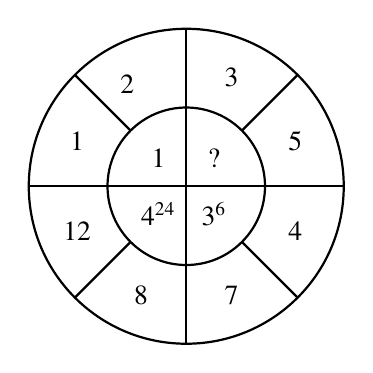
\begin{tikzpicture}


\draw[thick, black] (0, 0) circle (2);


\draw[thick, black] (0, 0) circle (1);



\draw[thick, black] (0, 0) -- (0:2);
\draw[thick, black] (0, 0) -- (90:2);
\draw[thick, black] (0, 0) -- (180:2);
\draw[thick, black] (0, 0) -- (270:2);

\node at (157.5:1.5) {1};
\node at (120:1.5) {2};
\node at (67.5:1.5) {3};
\node at (22.5:1.5) {5};
\node at (-22.5:1.5) {4};
\node at (-67.5:1.5) {7};

\node at (-112.5:1.5) {8};
\node at (-157.5:1.5) {12};


\node at (-135:0.5) {$4^{24}$};
\node at (-45:0.5) {$3^6$};
\node at (135:0.5) {1};
\node at (45:0.5) {?};
\draw[thick,black] (45:2) -- (45:1);
\draw[thick,black] (135:2) -- (135:1);
\draw[thick,black] (-135:2) -- (-135:1);
\draw[thick,black] (-45:2) -- (-45:1);


\end{tikzpicture}   \end{center}   

\item Let $z_1, z_2$ be the roots of the equation $z^2 + az + 12 = 0$ and $z_1, z_2$ form an equilateral triangle with the origin. Then, the value of $\abs{a}$ is \underline{\hspace{1cm}}.\hfill (March 2021)
\\

\item The number of solutions of the equation $\abs{\cot x}  = \cot x + \frac{1}{\sin x}$ in the interval \sbrak{0, 2\pi} is \underline{\hspace{1cm}}\hfill (March 2021)
\\

\item Let the plane $ax + by + cz + d = 0$ bisect the line joining the points $\brak{4, -3, 1}$ and $\brak{2, 3, -5}$ at right angles. If $a, b, c, d$ are integers, then the minimum value of $\brak{a^2 + b^2 + c^2 + d^2}$ is \underline{\hspace{1cm}}. \hfill (March 2021)
\\
\item If $f(x) = \int \frac{5x^8 + 7x^6}{(x^2 + 1 + 2x^7)^2} \, dx$, $\brak{x \geq 0}$, $f(0) = 0$ and $f(1) = \frac{1}{k}$, then the value of $k$ is \underline{\hspace{1cm}}\hfill (March 2021)




\end{enumerate}


\end{document}
